% confusion matrix
Confusion matrix is shown in Figure.\ref{fig:confusion_matrix}. We notice that several
pairs of categories are relatively easier to be confused and misclassified by the
SVMs with each other, such as bakery and deli, living room and bedroom, as well as
bookstore and library. We show some sample training and testing images from these
pairs in Figure~\ref{fig:sample}. For the bakery and deli pair, they both contain very
similar patterns of breads and sandwiches on shelves. For the livingroom and bedroom
pair, some living room images may include bed or bed-like sofa, which is almost identical
to the beds and sofas in images from bedroom category. For the library and bookstore,
both contain identical shelves of books. It is very difficult, even for human beings, to distinguish
images between these two categories.

\begin{figure*}[ht]
  \centering
  \includegraphics[width=1.0\textwidth]{img/matrix.pdf}
  \centering
  \label{fig:confusion_matrix}
\end{figure*}

% sample image from dataset

\begin{figure*}[ht]
  \centering
  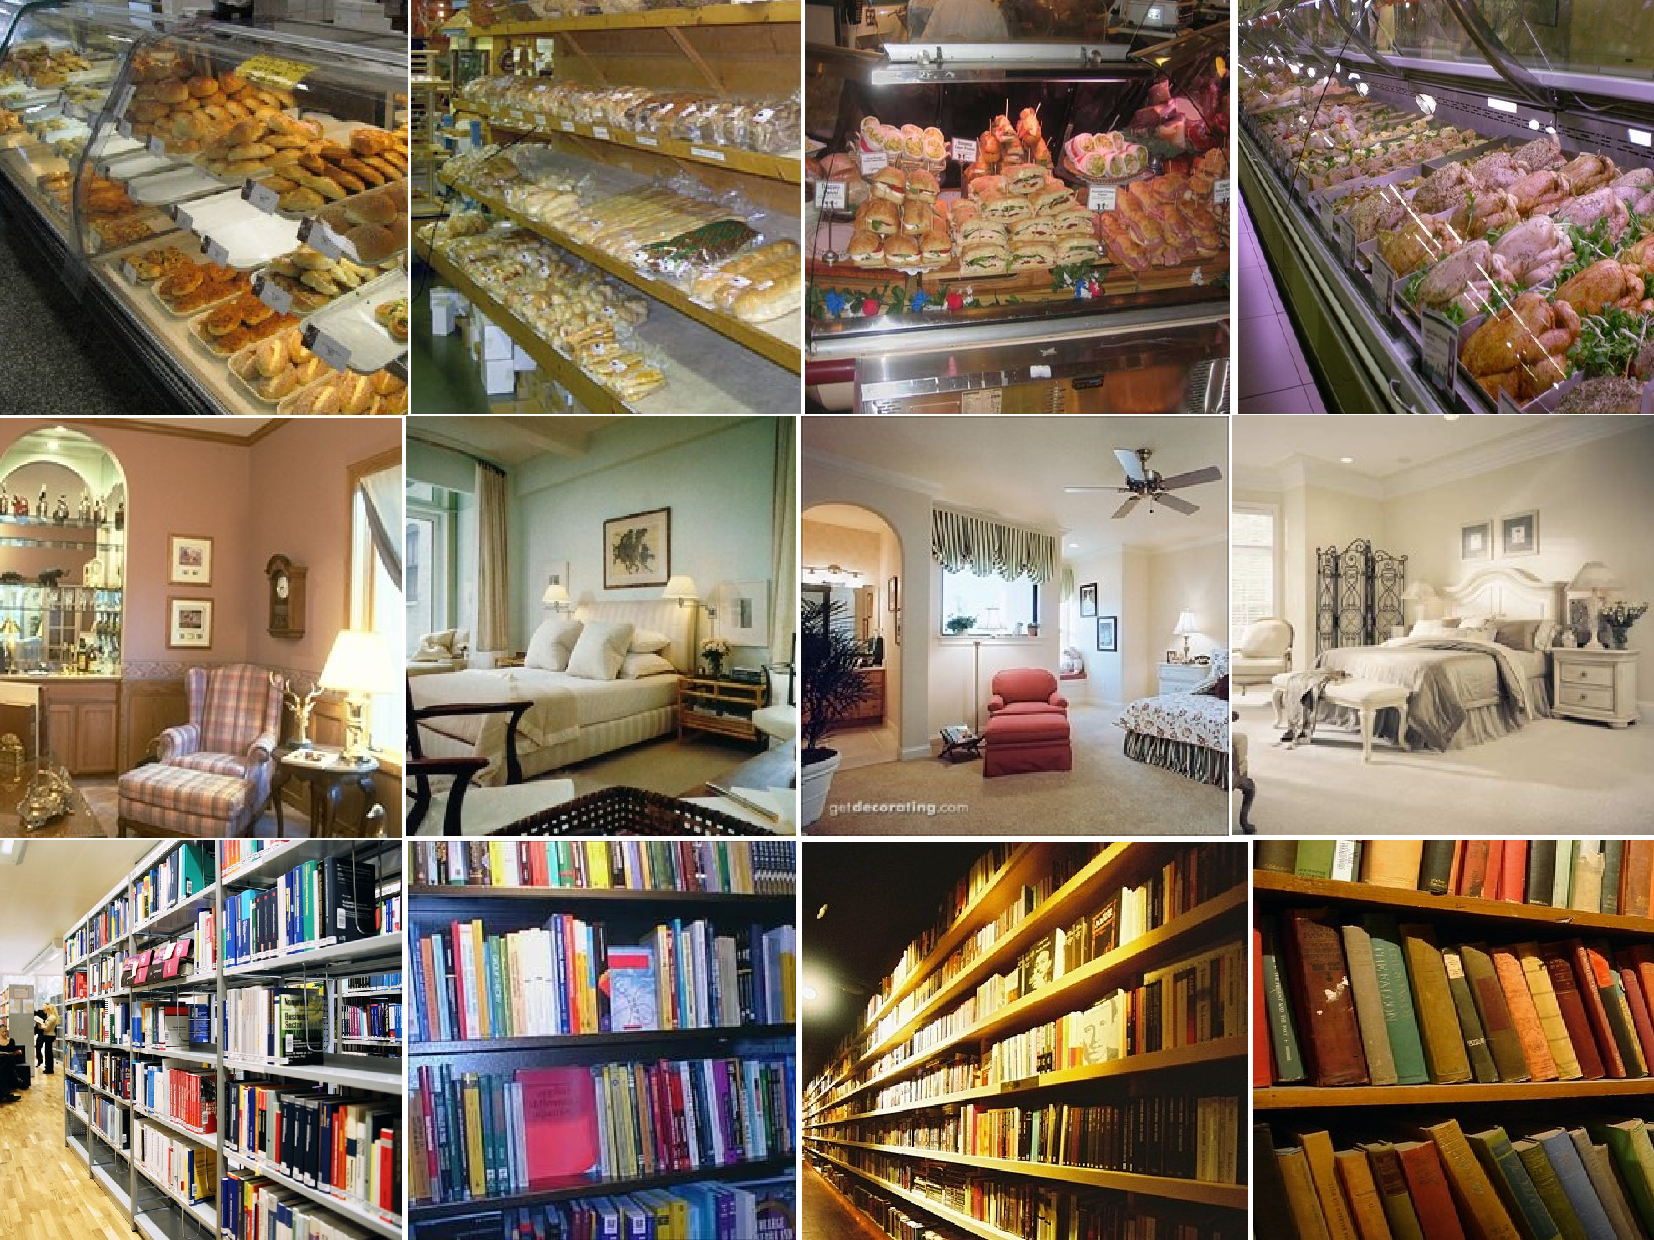
\includegraphics[width=0.8\textwidth]{img/dataset.pdf}
  \centering
  \caption{This figure contains some sample images from the MIT-indoor67 dataset.
For each row, left two columns are from the same category and right two columns are from
another. The first pair is bakery and deli, the second pair is living rooms and bedrooms, and the last pair is library and bookstore.}
\label{fig:sample}
\end{figure*}
